\subsection*{Control Model}
In order to implement the adaptive control in the Julia programming language, we needed a way to account for the adaptation law. This implementation was not initially very straightforward, as the ``simulate!()" function places certain restrictions on the inputs to the control function that we choose. To alleviate this issue, we made the adaptive controller a mutable structure which contains the adaptation parameter as a member. This implementation allows us to continually update the parameter, without having to troubleshoot issues associated with other methods.\\

With this control fully implemented, we then move to the full simulation of the control in which we track the state error and end-effector trajectory.
\begin{figure}[H]
	\centering
	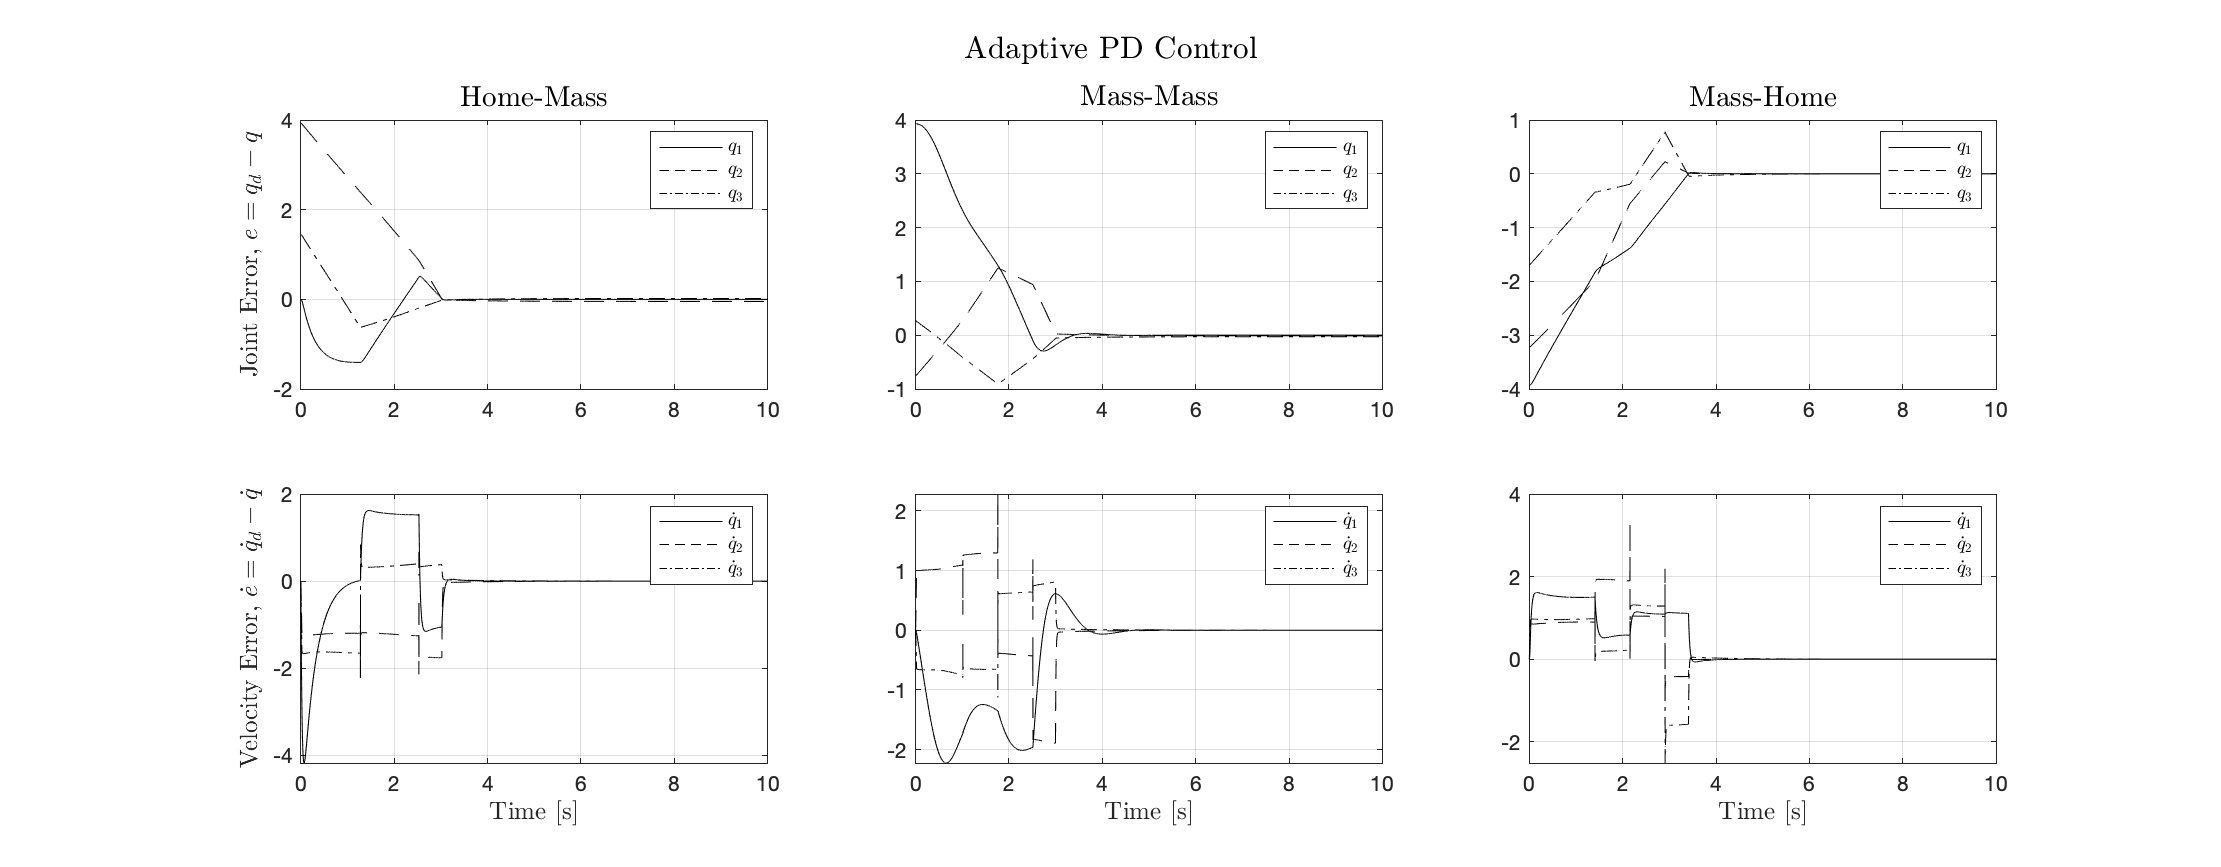
\includegraphics[width=\textwidth]{figures/mass10NNerrAPD.eps}
	\caption{Adaptive controller error in full simulation}
	\label{fig:nnerrapd}
\end{figure}
\begin{figure}[H]
	\centering
	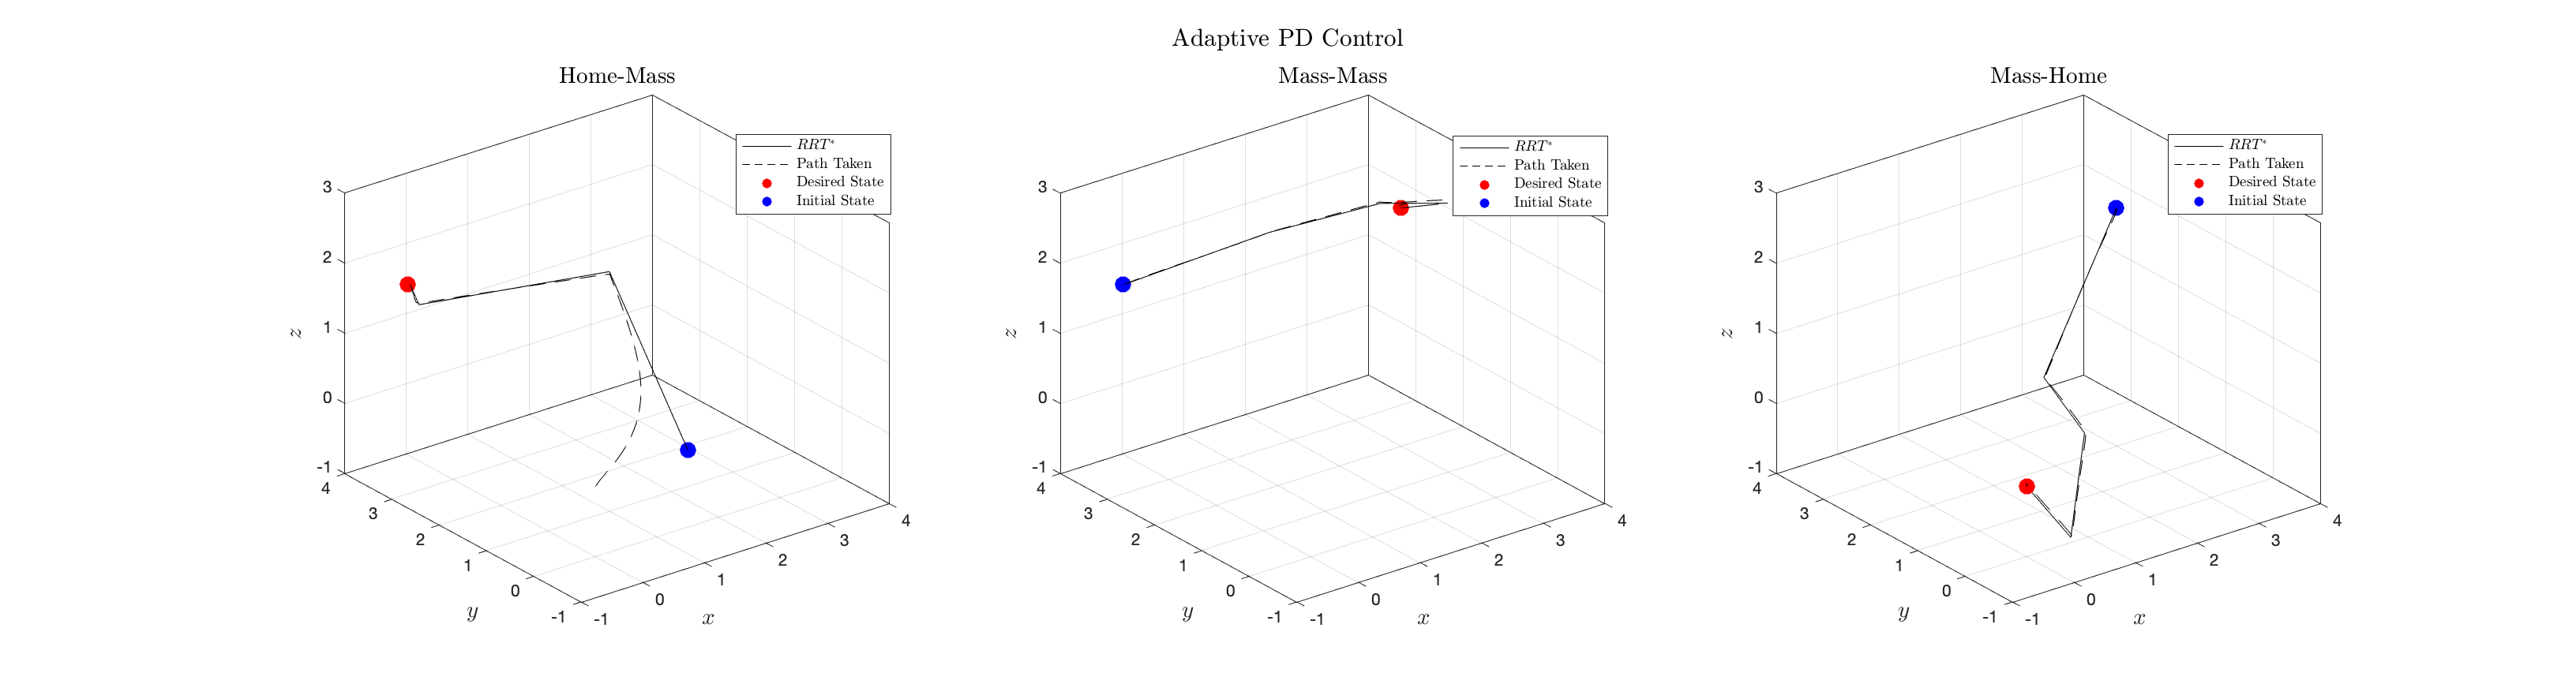
\includegraphics[width=\textwidth]{figures/mass10NNeetrajAPD.eps}
	\caption{End-effector trajectory with adaptive control}
	\label{fig:nntrajapd}
\end{figure}
We can see from Fig. \ref{fig:nntrajapd} that our initial error results in a false start position, however this error quickly decreases to zero as expected, and the trajectory is followed very tightly for the remainder of the simulation. We then look at a strict PD model, to observe the effects that an increase in mass has on the control.
\begin{figure}[H]
	\centering
	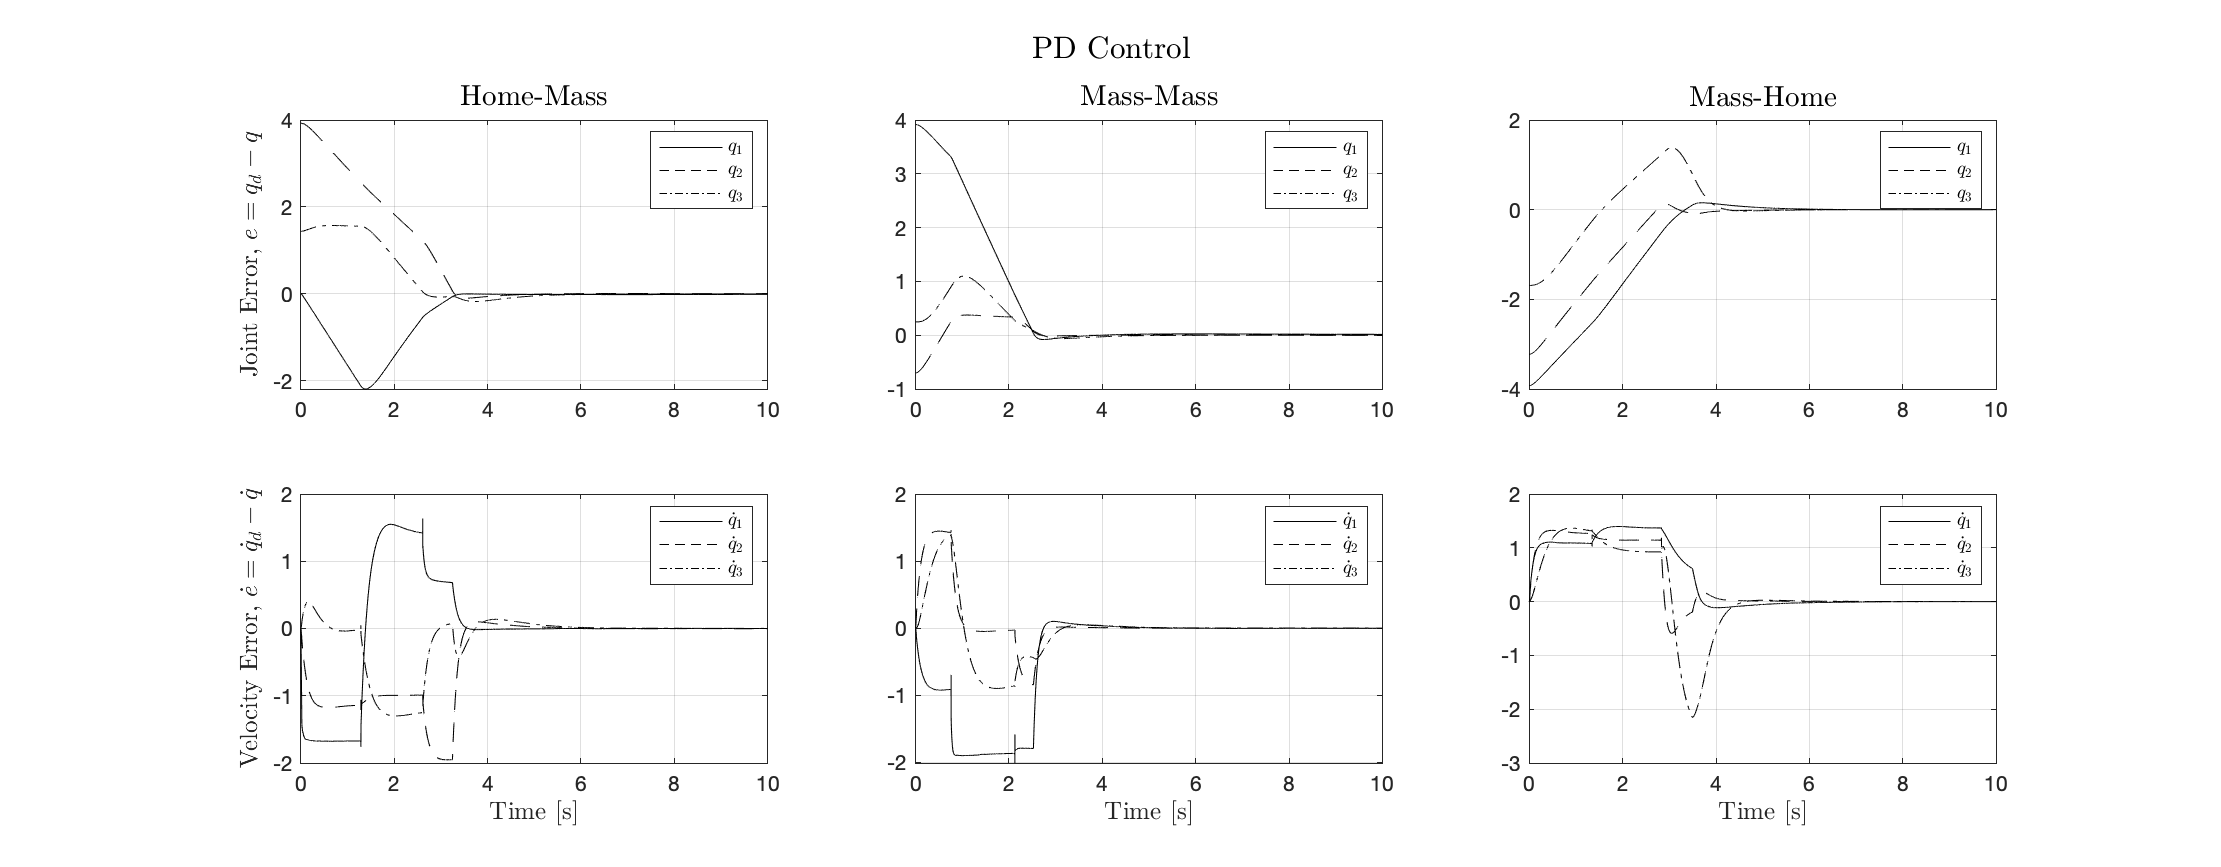
\includegraphics[width=\textwidth]{figures/mass10NNerrPD.eps}
	\caption{PD controller error in full simulation}
	\label{fig:nnerrpd}
\end{figure}
\begin{figure}[H]
	\centering
	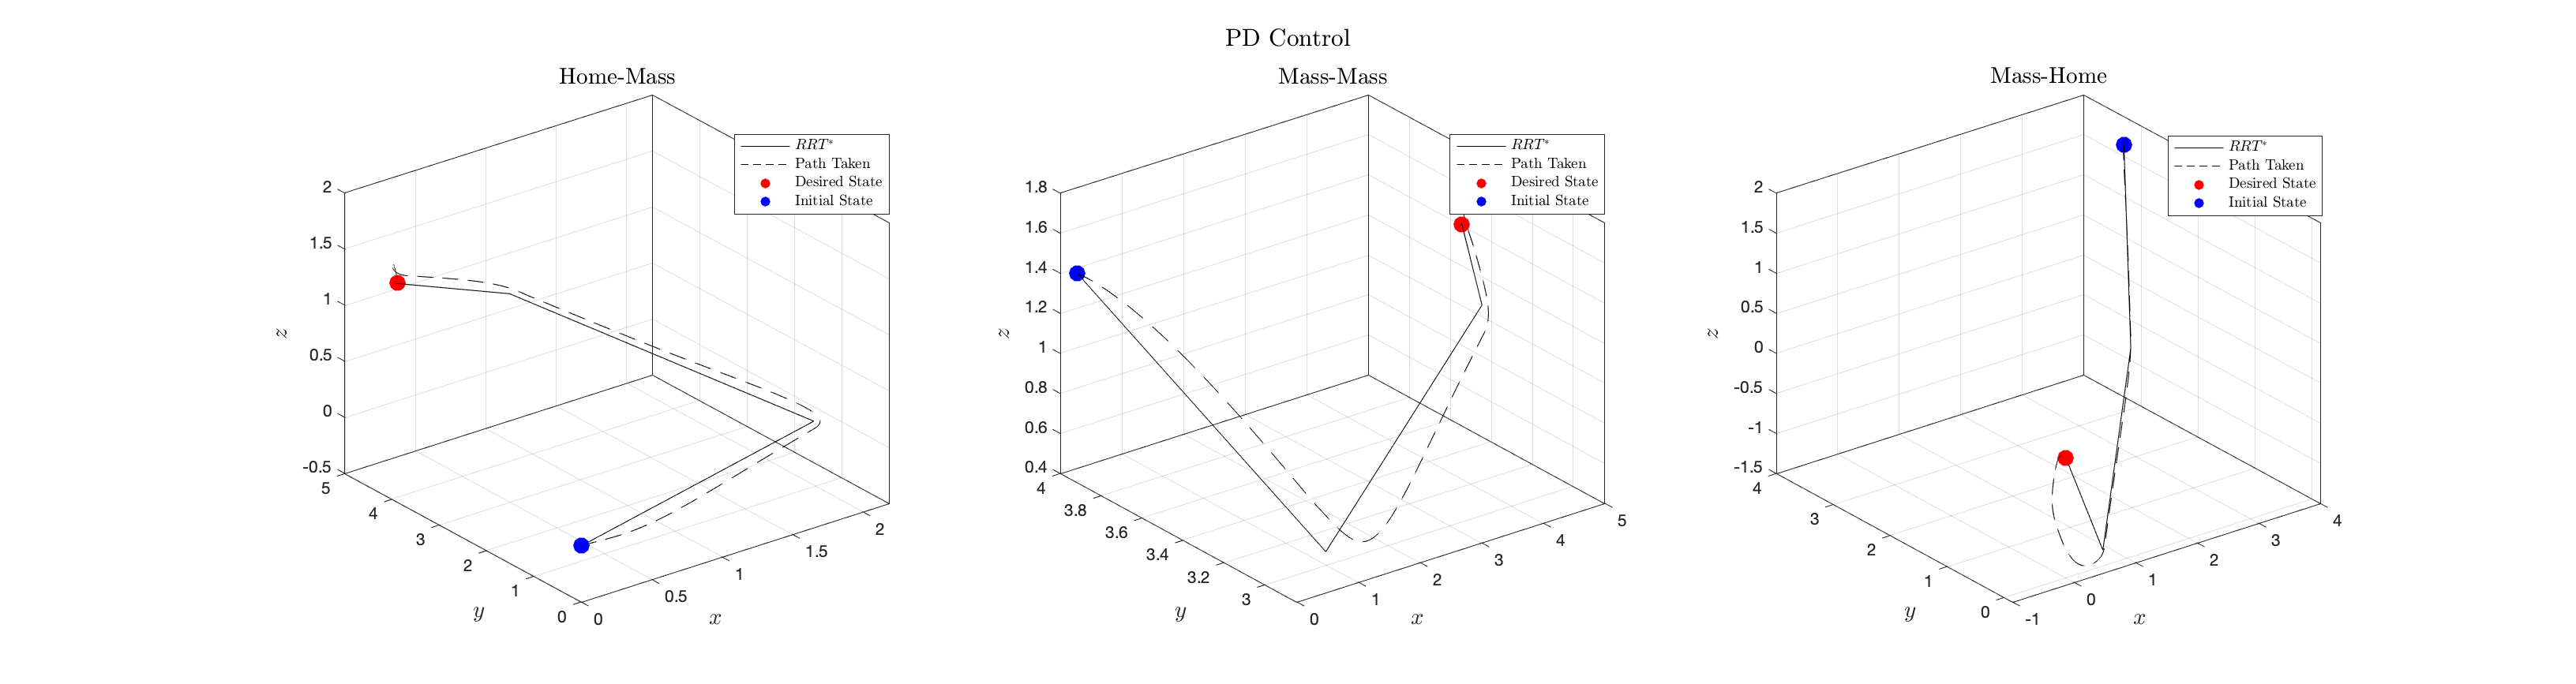
\includegraphics[width=\textwidth]{figures/mass10NNeetrajPD.eps}
	\caption{End-effector trajectory with PD control}
	\label{fig:nntrajpd}
\end{figure}
In contrast to the adaptive model, the PD controller places the end-effector in the desired start position. However, we can easily see from Fig. \ref{fig:nntrajpd} that the PD control is not able to follow the desired trajectory as closely, and once the mass is picked up this issue worsens.